\section[Specyfika testowanych Urządzeń]{Specyfika testowanych Urządzeń}
Ze względu na ograniczenia związane ze zużyciem energii, urządzenia mobilne są nie często wykorzystywane do większych zadań obliczeniowych. Zwykle praca procesorów graficznych wykorzystywana jest głównie do wspierania aplikacji graficznych. Procesory Graficzne działają w modelu przetwarzania pojedynczą instrukcją kilku elementów pamięci (SIMD). Tak by móc jedną instrukcją w tym samym czasie wykonać operacje na przykład na kilku pixelach z obrazka. 
\begin{figure}[H]
	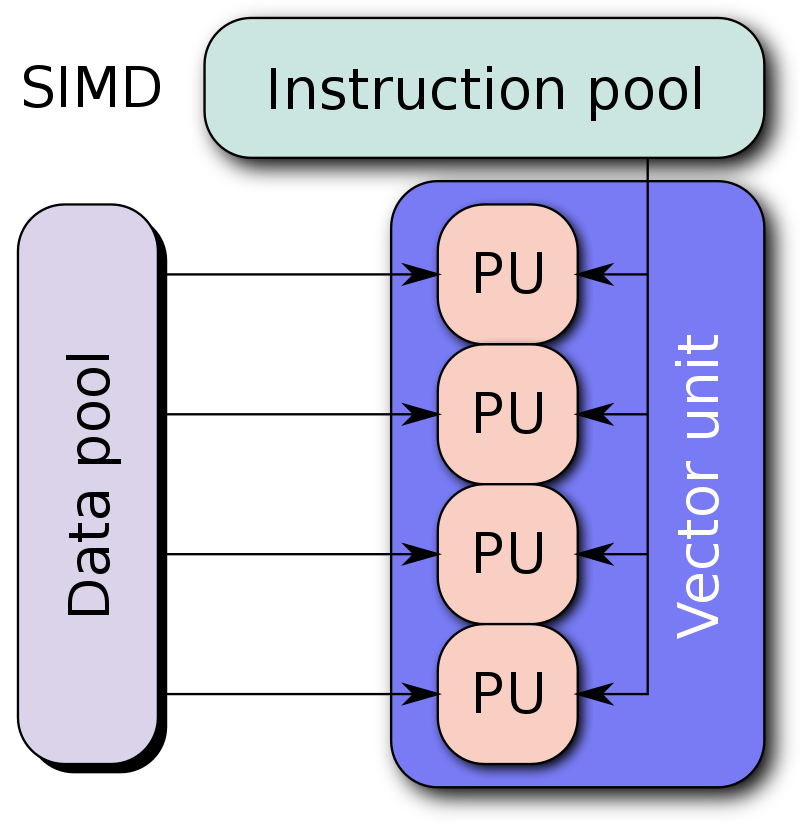
\includegraphics[scale=0.16]{imgs/SIMD2.svg.png}
	\caption{SIMD \cite{SIMD}}
\end{figure}

\subsection[Porównanie Graficznych Procesorów Mobilnych]{Porównanie Graficznych Procesorów Mobilnych}
Dwoma głównymi producentami procesorów graficznych na mobilne platformy są Qualcomm produkujący procesory Adreno i ARM tworzący GPU o nazwie Mali. 
Oto podstawowe wady i zalety, które odróżniają wymienione produktu
\begin{itemize}
	\item \textbf{Wydajność:} Urządzenia Adreno w większości przypadków osiągają lepsze wyniki performancowe. Dla proównywalnych modeli Adreno 660 i Mali-G78 MP24 ten pierwszy osiąga 1486 GFLOPS, a drugi tylko 1076 GFLOPS.
	\item \textbf{Wsparcie api:} Sarsze urządzenia adreno posiadają wsparcie dla szerszej api w nowszych wersjach. Najnowsze modele procesorów Mali, wspierają podobną liste api.
	\item \textbf{Częstotliwość zegara:} W większości przypadków procesory Mali posiadają wyższe częstotliwości zegara od konkurentów. Procesor Mali G51 pracuje z częstotliwością 1 GHz. Pośród produktów Adreno, żaden nie osiąga takiej wartości.
	\item \textbf{Cena:} Qualcom jest frmą z USA, która nażuca większe koszty licencyjne swoich układów dla producentów telefonów. Sprawia to, że układy Mali częsciej znajdą się w tańszych urządzeniach.
	\item \textbf{Renderowanie:} w tej kategorii układy Mali mają dużą przewagę nad Adreno. Przykładowo procesor Adreno 660 jest wstanie renderować 1524 milionów trójkątów na sekundę, a konkurencyjny Mali G78 MP24 moze ich wyrenderować 2463 w tym samym czasie.
	\item \textbf{Problem z odprowadzaniem ciepła:} Jako, że procesory Mali działają z wyższym taktowaniem zegara, często dochodzi do przegrzania układów. Dzięki niższej temperaturze procesory Adreno mogą być bardziej wydajne.
\end{itemize}
\begin{table}[H]
    \caption{Bezpośrednie porównanie wad i zalet procesorów Mali i Adreno}
    \label{tab:skale}
    \begin{tabular}{|l|c|c|}
\hline
Cecha & Adreno & Mali\\
\hline
Wydajność & + & -\\
\hline
Cena & - & + \\
\hline
Wsparcie Api & + & -\\
\hline
Częstotliwość zegara & - & +\\
\hline
Renderowanie & - & +\\
\hline
Przegrzewanie & + & -\\
\hline
\end{tabular}
\end{table}
	
	
\subsection[Urządzenia wykorzystane do testowania]{Urządzenia wykorzystane do testowania}
\subsubsection[Xiaomi Mi A2 Lite]{Xiaomi Mi A2 Lite}
Jest to telefon z lipca 2018 roku. Posiadający ośmiordzeniowy procesor Cortex A53, z częstotliwością zegara 2.0GHz. Pamięć systemowa urządzenia to 3GB. Umieszczono w nim Procesor graficzny Adreno 506. Procesor ten posiada 96 jednostek mogących jednocześnie wykonywać wątki na urządzeniu. Częstotliwość zegara procesora wynosi 650MHz. Dodatkowo posiada on 128 KB pamięci wbudowanej w chip GPU oraz 8 KB pamieci cache. Wykorzystuje pamięć typu LPDDR3 933MHz i przepustowości 7.4GB/s. Wspiera następujące api: Vulkan 1.0, OpenGL 3.2, DX11, OpenCL 2.0. Telefon Posiada system operacyjny Android w wersji 10. Sterownik OpenCL na urządzeniu jest w wersji \#7331a27 z 11/13/19, posiada wsparcie dla typu zmiennoprzecinkowe Half, oraz dla współdzielenia zasobów z OpenGL. Nie posiada wsparcia dla typów zmiennoprzecinkowych podwójnej precyzji Double.
\subsubsection[Huawei P20 Lite]{Huawei P20 Lite}
Jest to Urządzenie z marca 2018 roku. Wyposażone jest w 8 rdzeniowy procesor 4x2.36 GHz Cortex-A53 + 4x1.7 GHz Cortex-A53. Posiada on 4GB pamięci systemowej. Wbudowany procesor graficzny to Mali-T830 MP2, procesor posiada dwie jednostki wykonawcze, pojedyncza jednostka w tym procesorze może wykonywać 32 wątkói. Częstotliwość zegara wynosi 9000MHz, posiada 16KB pamięci cache. Korzysta z pamięci typu LPDDR3 o częstotliwości 933MHz i przepustowości do 14.9 GB/s. Wspiera następujące api: Vulkan 1.0, OpenCL 1.2, OpenGL 3.2. Wspiera typ Half oraz Double, nie wspiera współdzielenia zasobów z OpenGL. Telefon działa z systemem operacyjnym Android w wersji 9
\subsubsection[HTC Desire 820]{HTC Desire 820}
Telefon z 2014 roku, wyposażony w procesor ośmiordzeniowy 1,7 GHz quad-core Cortex-A53 + 1 GHz quad-core Cortex-A53. Posiada 2GB pamięci RAM. Posiada procesor graficzny Adreno 405. Gpu może wykonywać na raz 48 wątków, dodatkowo posiada 256KB pamięci dedykowanej. Wykorzystano pamięć typu LPDDR3 z częstotliwością 666.5MHz i szybkości 5.3GB/s Wspierane przez urządzenia api to: OpenGL 3.2, OpenCL 1.2, DX11. Telefon Dla Systemu Android w wersji 5 posiada sterownik OpenCL w wersji z 29.04.15, a z androidem 6 w wersji z 23.03.2016. Wspiera typ Half, nie wspiera Double, możliwe do wykorzystania rozszerzenie współdzielenia zasobów między OpenCL i OpenGL.
\subsubsection[Xiaomi Redmi Note 7]{Xiaomi Redmi Note 7}
Telefon wydany na początku 2019 roku. Posiada procesor ośmiordzeniowy Qualcomm Kryo 260 z częstotliwością do 2,2 GHz. Wyposażony w 6GB pamięci systemowej. Dodatkowo posiada Procesor graficzny Adreno 512. GPU działa z częstotliwością 850MHz posiada 256KB pamięci dedykowanej i 16KB cache, pamięć typu LPDDR4 o częstotliwości 1866MHz i przepustowości do 29.8GB/s. Może wykonywać na raz 128 wątków. Telefon działa z systemem android w wersji 10, posiada sterownik OpenCL w wersji:\#9b15012 z 09/17/20.Wspiera api Vulkan 1.0, OpenGL 3.2, DX11, OpenCL 2.0. OpenCL nie wspiera typu double, ale wspiera typ Half oraz współdzielenie zasobów z OpenGL.
\subsubsection[Samsung Galaxy A70]{Samsung Galaxy A70}
To urządzenie, którego premiera odbyła się na początku 2019 roku. wyposażony w procesor ośmiordzeniowy Kryo 460 z częstotliwością zegara do 2 GHz. Posiada 6GB pamięci RAM. Dodatkowo posiada procesor graficzny Adreno 612 o częstotliwości 845Mhz, 128 wątkach, wbudowanej pamięci 256KB i 16KB pamięci cache, jest to pamięć typu LPDDR4X o częstotliwości 1866MHz i przepustowości do 14.9GB/s. Android w wersji 10 ze sterownikiem OpenCL w wersji \#e1ac91e z 11/17/20. Wspiera typ Half, nie wspiera Double, możliwe do wykorzystania rozszerzenie współdzielenia zasobów między OpenCL i OpenGL.
\subsubsection[Porównanie]{Porównanie}
Zdecydowanie urządzeniem z najsłabszymi parametrami jest HTC Desire 820. Xiaomi Mi A2 Lite oraz Huawei P20 lite posiadają konkurencyjne parametry, jednak są urządzeniami posiadające podzespoły od różnych producentów. Najmocniejszymi są Redmi Note 7, który ma najszybszą pamięć oraz najszybciej pracujący procesor, oraz SAmsung Galaxy A70, który ma najnowszy procesor graficzny.

\begin{table}[H]
    \caption{Porównanie testowanych telefonów}
    \label{tab:skale}
    \begin{tabular}{|l|c|c|c|c|}
\hline
\textbf{Telefon} & \textbf{Data wydania} & \textbf{CPU} & \textbf{RAM} & \textbf{GPU}\\
\hline
Xiaomi Mi A2 Lite & Q3 2018 & \makecell{8x Cortex-A53 \\ do 2 GHz} & 3GB & Adreno 506\\
\hline
HTCDesire 820 & Q3 2014 & \makecell{1,7 GHz quad-core Cortex-A53 + \\ 1 GHz quad-core Cortex-A53} & 2GB & Adreno 405 \\
\hline
Huawei P20 Lite & Q2 2018 & \makecell{4x2.36 GHz Cortex-A53 + \\ 4x1.7 GHz Cortex-A53} & 4GB & Mali T830 MP2 \\
\hline
Samsung Galaxy A70 & Q1 2019 & \makecell{8x Kryo 460 \\ do 2 GHz } & 6GB & Adreno 612 \\
\hline
Xiaomi Redmi Note 7 & Q1 2019 & \makecell{8x Qualcomm Kryo 260 \\ do 2,2 GHz} & 6GB & Adreno 512 \\
\hline
\end{tabular}
\end{table}
\begin{table}[H]
    \caption{Porównanie dostępnosci api na testowanych urządzeniach}
    \label{tab:skale}
    \begin{tabular}{|l|c|c|c|c|c|c|}
\hline
\textbf{GPU} & \textbf{Vulkan} & \textbf{D3D} & \textbf{OpenCL} & \textbf{OGL} & \makecell{\textbf{Data kompilacji} \\ \textbf{sterownika OpenCL}} & \makecell{\textbf{Wspierane} \\ \textbf{rozszeżenia}}\\
\hline
Adreno 506 & 1.0 & DX11 & 2.0 & 3.2 & 13.11.2019r. & \makecell{cl\_khr\_gl\_sharing \\ cl\_khr\_fp16}\\
\hline
Adreno 405 & N/A & DX11 & 1.2 & 3.2 & 23.03.2016r. & \makecell{cl\_khr\_gl\_sharing \\ cl\_khr\_fp16}\\
\hline
Mali T830 2MP & 1.0 & DX11 & 1.2 & 3.2 & N/A & \makecell{cl\_khr\_fp64 \\ cl\_khr\_fp16}\\
\hline
Adreno 612 & 1.1 & DX12 & 2.0 & 3.2 & 17.11.2020r. & \makecell{cl\_khr\_gl\_sharing \\ cl\_khr\_fp16}\\
\hline
Adreno 512 & 1.0 & DX11 & 2.0 & 3.2 & 17.09.2020r. & \makecell{cl\_khr\_gl\_sharing \\ cl\_khr\_fp16}\\
\hline
\end{tabular}
\end{table}

\begin{table}[H]
    \caption{Porównanie testowanych procesorów graficznych}
    \label{tab:skale}
    \begin{tabular}{|l|c|c|c|c|}
\hline
\textbf{GPU} & \makecell{\textbf{Częstotliwość} \\ \textbf{zegara}} & \textbf{Pamięć} & \makecell{\textbf{Typ} \\ \textbf{pamięci}} & \makecell{\textbf{Ilość jednostek} \\ \textbf{wykonawczych}}\\
\hline
Adreno 506 & 650 MHz & 128 KB + 8 KB & \makecell{LPDDR3-1866 \\ 933 MHz 7.4 GB/s} & 96\\
\hline
Adreno 405 & 550 MHz & 256 KB & \makecell{LPDDR3-1333 665.5 MHz \\ 5.3 GB/s} & 48\\
\hline
Mali T830 2MP & 900 MHz & 128KB & \makecell{LPDDR3 \\ 933MHz} & 2 x 32\\
\hline
Adreno 612 & 845 MHz & 256KB + 16KB & \makecell{LPDDR4X-3732 1866 MHz \\ Dual chanel 16 bit \\ 14.9 GB/s} & 128\\
\hline
Adreno 512 & 850 MHz & 256KB + 16KB & \makecell{LPDDR4-3732 1866 MHz \\ Quad chanel 16 bit \\ 29.8 GB/s} & 128\\
\hline
\end{tabular}
\end{table}

